\section{Monads in the Wild}
\subsection{Overview}
Typically a programmer will think of a monad as three function signatures
which correspond to the triple $(T,\eta,\mu)$;
of course much more informally.
Firstly \texttt{fmap} corresponds to the functor $T$,
then we have \texttt{return} and \texttt{join} which correspond to
the natural transformations $\eta$ and $\mu$ respectively.
We should note that the terms \texttt{fmap,return,join}
are not fixed, relatively often other names are used;
for example \texttt{map} instead of \texttt{fmap}
or \texttt{pure/unit} instead of \texttt{return},
however the semantics are exactly the same.

\begin{equation}
  \begin{split}
    fmap   &:: (x \rightarrow y) \rightarrow M x \rightarrow M y \\
    return &:: x \rightarrow M x                                 \\
    join   &:: M (M x) \rightarrow M x
  \end{split}
\end{equation}

To be a correct monad implementation it must be true that:
\begin{equation}
  \begin{split}
      \lambda f.\lambda x.return\ (fmap\ f\ x)
      &\equiv
      \lambda f.\lambda x.fmap\ (return \circ f)\ x)
      \\
      \lambda f.\lambda x.fmap\ f\ x
      &\equiv
      \lambda f.\lambda x.fmap\ f\ (fmap\ id\ x)
      \\
      \lambda f.\lambda x.join\ (join\ (fmap\ f\ x))
      &\equiv
      \lambda f.\lambda x.join(fmap\ f\ (join\ x))
  \end{split}
\end{equation}

Contrast these monad implementation laws with the diagrams
\begin{equation}
    \begin{tikzcd}[sep=large]
        T \rar{\eta_T} \drar[swap]{1_{C}} & T^2 \dar{\mu} & \lar[swap]{T\eta} \dlar{1_{C}} T \\
                                           & T            &
    \end{tikzcd}
    \quad
    \begin{tikzcd}[sep=large]
        T^3 \rar{T\mu} \dar[swap]{\mu_T} & T^2 \dar{\mu} \\
        T^2 \rar[swap]{\mu}                    & T
    \end{tikzcd}
\end{equation}

Do monad implementations need to follow these axioms?
There is no way for the compiler to check these rules so practically the answer is no,
however it is wise for monad implementations to obey them so that
we can chain computations in predictable and understandable ways.

%For programmers the most important of the triple is \texttt{fmap},
%this is because it is our primary way to interact with the monad.
%Typically we describe our desired result in terms of functions on the monad
%done one after the other.
However we can create a new function from this triple
\begin{align}
    bind &:: M x \rightarrow (x \rightarrow M y) \rightarrow M y \\
    bind &\equiv \lambda mx. \lambda f. join(fmap\ f\ mx)
\end{align}
Bind is incredibly useful and perhaps more prominent
to a programmer than the triple $(fmap,return,join)$.
This is because it allows us to chain computations
one after the other.
\begin{equation}
    x\
    \stackrel{f}{\rightarrow} My
    \stackrel{g}{\rightarrow} MMz
    \stackrel{join}{\rightarrow} Mz
\end{equation}
\begin{equation}
    \lambda g.
    \lambda f.
    \lambda x.
    join\ (fmap\ g\ (fmap\ f\ x))
\end{equation}
\begin{equation}
    (fmap\ f\ x) >>= g
\end{equation}

It is convention to use bind as the infix operator "$\bind$".
Consider that \texttt{join} can be expressed in terms of \texttt{bind} (with \texttt{id})
\begin{equation}
    join\ m \equiv m \bind id
\end{equation}
and furthermore so can \texttt{fmap} (with \texttt{return}).
\begin{equation}
    fmap\ f\ x \equiv (return\ x) \bind f
\end{equation}

%TODO bind relation to kleisli cat
Can we consider bind as a morphism between two objects in the Kleisli Category?

Because \texttt{bind} is often found with \texttt{(fmap,join,return)},
we can reformulate our axioms in terms of bind;
indeed the axioms are often reformulated this way because it is simpler.
\begin{align}
    return\ x \bind f &\equiv f x \\
    m \bind return &\equiv m \\
    (m \bind f) \bind g &\equiv m \bind (\lambda x.(f\ x \bind g))
\end{align}

We can further rephrase these axioms in terms
of the \textit{Kleisli composition operator} $\gg$ where
\begin{align}
    \gg &:: (x \rightarrow M y) \rightarrow (y \rightarrow M z) \rightarrow (x \rightarrow M z) \\
    f \gg g &\equiv \lambda x. (f\ x) >>= g
\end{align}
and we have
\begin{equation}
    (f \gg g) \gg h \equiv f \gg (g \gg h)
\end{equation}
\begin{equation}
    return \gg f \equiv f \equiv f \gg return
\end{equation}

\subsection{Monads for Structuring Programs}
In this section I will illustrate how effective monads are when used to structure programs.

It is well accepted that some algorithms become much more elegant
and simple when expressed in a functional paradigm

Firstly one should note that OCaml has non-nullable types
i.e; one will never see null or nil where one is expecting an
int or a binary tree or anything else.
Null values are always explicit.
The canonical representation of null is the None variant.
Monads can be used to succinctly and expressively structure computation with the option type.
%TODO Elucidate non-nullable types
%TODO Explain maybe
%Why is this?
%Why do we need monads to this?
%What do other languages do?

\begin{verbatim}
  type 'a option = Some 'a | None
  val return : 'a -> 'a option
  val join   : 'a option option -> 'a option
  val fmap   : 'a option -> ('a -> 'b) -> 'b option
\end{verbatim}

The code for these three functions is simple and fairly self-evident.
For example here is \texttt{join} for all values:
\begin{verbatim}
    join None            = None
    join (Some None)     = None
    join (Some (Some x)) = Some x
\end{verbatim}

However from this simple basis we can construct much more complicated programs which we
will be certain will never have a \textit{NullPointerException}.
Furthermore the type system will ensure 
It will refuse to compile nonsensical code which does not account for none
wherever it is possible to see none.
Such an assurance is invaluable in creating correct programs.
Here it's important to note that the effect is the \textit{NullPointerException};
we deal with it much more cleanly and effectively 100\% of the time using monads.

\begin{verbatim}
  let return a = Some a
  let join = function
      | Some (Some a) -> Some a
      | _ -> None
  let fmap a f = match a with
      | None -> None
      | Some x -> Some (f x)
\end{verbatim}

Consider this example code for searching a trie data structure.
Briefly, a trie is key value data structure;
where the key is a finite sequence of values
(typically a string which is equivalent to a sequence of characters).
Each node has an option value and a list of children.
The root of the trie represents the empty string.
Two auxiliary functions \texttt{find\_child} and \texttt{val\_extract}
are used in the search code; \texttt{val\_extract}
simply returns the first value in a pair,
find child searchs the list of children returning
the node with the matching character given;
that is only should that child exists.

\begin{verbatim}
  type ('k, 'v) t = Trie of 'v option * (('k * ('k, 'v) t) list)
  val find_child  : ('k, 'v) t -> 'k -> ('k, 'v) t option
  val val_extract : ('k, 'v) t -> 'v option
  val create      : 'k list -> 'v -> ('k, 'v) t
  val get         : ('k, 'v) t -> 'k list -> 'v option

  let create key data =
    let rec aux = function
      | []      -> Trie (Some data, [])
      | c :: cs -> Trie (None, [(c, aux cs)])
    in aux key
\end{verbatim}

Create is shown to just illustrate the data structure,
we simply iterate across the list creating a node in the trie for each character
until the list is exhausted at which point we insert the value.

Below is an example of a trie,
mapping list of characters to intergers,
at the root is the empty string,
then we have various key value pairs,
for example the key "tea" has the value 6.
Note that although "te" is part of the trie,
it has no value associated with that key.
Also note that keys not at leaf level can have associated
values, for example ("in", 4).
\begin{center}
    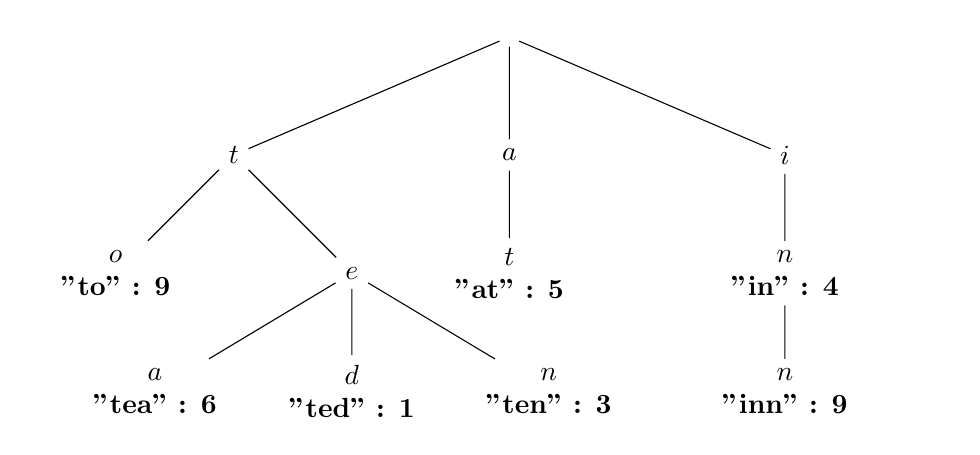
\begin{tikzpicture}[level distance=1.5cm,
  level 1/.style={sibling distance=3.5cm},
  level 2/.style={sibling distance=3cm},
  level 3/.style={sibling distance=2.5cm}]
  \node {$\varnothing$}
        child {node {$t$}
            child {node[text width=2cm,align=center] {$o$ \\ \textbf{"to" : 9}}}
            child {node {$e$}
                child {node[text width=2cm,align=center] {$a$ \\ \textbf{"tea" : 6}}}
                child {node[text width=2cm,align=center] {$d$ \\ \textbf{"ted" : 1}}}
                child {node[text width=2cm,align=center] {$n$ \\ \textbf{"ten" : 3}}}
            }
        }
    child {node {$a$}
            child {node[text width=2cm,align=center] {$t$ \\ \textbf{"at" : 5}}}
        }
    child {node {$i$}
            child {node[text width=4cm,align=center] {$n$ \\ \textbf{"in" : 4}}
                child {node[text width=2cm,align=center] {$n$ \\ \textbf{"inn" : 9}}}
                }
    };
\end{tikzpicture}
\end{center}

In the search code t is the trie, key is a list of characters over which
we iterate the search function. For each character we call find child on
the current node. Find child, if succesful, will return the next node
upon which we continue the search with the remaining characters. Once we
are at the last character we know to try and extract the value from the end
node. The key point here is that using bind allows us to succintly only code
for the happy case but deal with the error case at every step.

\begin{verbatim}
  let get t key =
    let rec search chars t =
        match chars with
        | []      -> val_extract t
        | c :: cs -> bind_search (find_child t c) cs
    and bind_search ot chars = ot >>= search chars
    in search key t
\end{verbatim}

The result type is similar to the option type, however we use an extra type
parameter for the unhappy case, essentially the result type encapsulates 
either an error or a correct computation result. The result monad
corresponds to a generalisation of the exception monad presented by Wadler \cite{wadler1995monads}.

\begin{verbatim}
  type ('a, 'e) result = Ok of 'a | Error of 'e
  val bind : ('a, 'e) result
          -> ('a -> ('b, 'e) result)
          -> ('b, 'e) result
\end{verbatim}

In this example we have a list assocation which is a list of pairs, in this case both
items in the pairs are strings.

\begin{verbatim}
  let list_assoc_to_job la =
    let find k = match List.Assoc.find la k with
      | None -> Error (Err.missing_key k)
      | Some v -> Ok v
    in
    find "name"   >>=                  (fun name   ->
    find "prog"   >>=                  (fun prog   ->
    find "args"   >>= parse_args   >>= (fun args   ->
    find "run_at" >>= parse_run_at >>= (fun run_at ->
      Ok (Job.create name prog args run_at ())
    ))))
\end{verbatim}

Bind is used to succintly short circuit a computation when a value can not be
correctly obtained. As such this allows the program to be structured neatly to return
an error with precise information for which key could not be found or which value could
not be parsed. The result monad is very similar to the option monad. It would be interesting
to examine whether algebraic effects can be used to structure a program in a similar manner.

Typically programming languages allow the elison of the anonymous function on the right hand side
of the bind to simply introduce the binding into the environment;
in this case OCaml ppx extension points are used in the form \textit{let\%bind}.
This is largely just a programmer convienence,
for comparison Haskell offers \textit{do notation} for the same end.

\begin{verbatim}
  let list_assoc_to_job la =
    let find k = match List.Assoc.find la k with
      | None -> Error (Err.missing_key k)
      | Some v -> Ok v
    in
    let%bind name   =  find "name"                     in
    let%bind prog   =  find "prog"                     in
    let%bind args   = (find "args"   >>= parse_args  ) in
    let%bind run_at = (find "run_at" >>= parse_run_at) in
    Ok (Job.create name prog args run_at ())
\end{verbatim}
Is equivalent to
\begin{verbatim}
  let list_assoc_to_job la =
    let find k = match List.Assoc.find la k with
      | None -> Error (Err.missing_key k)
      | Some v -> Ok v
    in
    find "name"   >>=                  (fun name   ->
    find "prog"   >>=                  (fun prog   ->
    find "args"   >>= parse_args   >>= (fun args   ->
    find "run_at" >>= parse_run_at >>= (fun run_at ->
      Ok (Job.create name prog args run_at ())
    ))))
\end{verbatim}

In Haskell \texttt{do} is simply syntactic sugar for \texttt{>>=} and \texttt{>>} where
\begin{equation}
    \texttt{>> :: M x -> M y -> M y}
\end{equation}
i.e. do first and ignore the result and then do the second.
Consider it equivalent to the semi colon operator in imperative languages.
\begin{align}
    \texttt{do}\ \{ x;\ \texttt{<stmts>} \}
    &\equiv x \texttt{ >> do \{<stmts>\}}
    \\
    \texttt{do}\ \{ v \leftarrow x\ \texttt{ <stmts>}\}
    &\equiv x \texttt{ >>= } \lambda v.\ \texttt{do}\ \{ \texttt{<stmts>} \}
    \\
    \texttt{do}\ \{\texttt{let }x = v\ \texttt{<stmts>}\}
    &\equiv (\lambda x.\ \texttt{do}\ \{ \texttt{<stmts>} \})v
\end{align}

In this example we simply and effectively deal with two types of errors.
Firstly a key being missing from our list
\begin{verbatim}
    let find k = match List.Assoc.find la k with
      | None -> Error (Err.missing_key k)
      | Some v -> Ok v
\end{verbatim}
Secondly a more complicated value which we have to parse;
the parsing of which can fail
\begin{verbatim}
    let%bind run_at = (find "run_at" >>= parse_run_at) in
\end{verbatim}
The key point here is when we have an error we want to fail
loudly and give as much information as possible about why we failed.
Furthermore, we don't want to take care of that in this function
we don't want to put that logic here
Monads allow us to sequence this error handling
and keep the necessary logic in a sensible re-usable place.

Finally consider the relation between
\texttt{(let\%bind,do)} and the Kleisli category of programs.
Consider how convienent it is for programmers to have a category
of programs where reliable error handling is built in by default.

\subsection{State Monad Example}
In this section we will illustrate how closely
the $\lambda_c$-calculus relates to actual code,
similar to what is in the Haskell standard library.
Furthermore we will show that from the relatively
simple triple $(fmap,return,join) + bind$ we can
construct code which has effects.

Firstly recall our example \ref{lc1} computations with
side-effects\cite{moggi1989computational}:
\begin{itemize}
    \item $T(-)$ is the functor $(-\times S)^S$, where $S$ is a nonempty set of stores.
        Intuitively a computation takes a store and returns a value together with the modified store.
    \item $\eta_A$ is the map $a \rightarrow (\lambda s.\langle a,s \rangle)$
    \item $\mu_A$ is the map $f \rightarrow (\lambda s.eval(fs))$,
        i.e. $\mu_A(f)$ is the computation that given a store $s$,
        first computes the pair computation-store $\langle f\prime,s\prime\rangle = f\ s$
        and then returns the pair value-store $\langle a,s\prime\prime\rangle = f\prime\ s\prime$.
\end{itemize}

We will examine how this maps to the Haskell state monad,
this implementation is similar to the one in the standard library
and is inspired by \cite{jones1995functional}.
We need to begin by declaring the type of the state monad,
it is effectively a closure over a function
which takes a state \texttt{s} and returns a value \texttt{a}.
In Moggi's work the function is anonymous however we name it
\texttt{runState}.
\begin{verbatim}
    newtype State s a = State {runState :: s -> (a, s)}
\end{verbatim}

Next \texttt{return},
consider $\eta_A$ the map $a \mapsto (\lambda s.\langle a,s \rangle)$,
this is a straightforward translation,
we just return a closure to an anonymous function
which takes a state and returns the pair \texttt{(a,s)}.
This anonymous function becomes \texttt{runState} for our
monad $State\ a$.
\begin{verbatim}
    return a = State (\ s -> (a,s))
\end{verbatim}

Moggi defines $\mu_A$ as the map $f \rightarrow (\lambda s.eval(fs))$,
we define this
\begin{verbatim}
    join :: (State s (State s a)) -> (State s a)
    join ssa = State (\s ->
        let a, s' = (runState ssa) s in
        (runState s') a
    )
    -- More idiomatically
    join ssa = State (\s -> uncurry runState (runState ssa s))
    -- where
    uncurry :: (a -> b -> c) -> ((a, b) -> c)
    uncurry f = \p ->  f (fst p) (snd p)
\end{verbatim}

Next fmap, which Moggi defines as
the functor $(-\times S)^S$,
where $S$ is a nonempty set of stores.
This corresponds to applying $f$ to $a$ and
a new state $s\prime$.
\begin{verbatim}
fmap :: (a -> b) -> State s a -> State s b
fmap f m = State $ \ s -> (f a, s')
    where (a, s') = runState m s
\end{verbatim}

At this point we should consider
that the Haskell implementation is remarkably
similar to the definition specified by Moggi,
of course it is not a completely direct translation
however the relation is obvious.
That said, we have not yet defined something "usable",
but we are close.

Finally we can define \texttt{bind} as
\begin{verbatim}
    m >>= k = State $ \s -> case runState m s of
                        (a, s') -> runState (k a) s'
    -- Or rephrased slightly
    m >>= f  = State (\ s ->
        let (x, s') = runState m s in
        runState (f x) s')
\end{verbatim}

Briefly, one should note that it appears many Haskellers
have a terrible fear of extraneous parenthesis,
as such \texttt{\$} can be read as "\texttt{(}"
and put the matching "\texttt{)}" somewhere appropriate.

Recall that we proposed:
\begin{equation}
    join\ m \equiv m \bind id
\end{equation}
Now is an ideal time to verify this in practise,
replace \texttt{k} for \texttt{id} and
observe that $id\ x \equiv x$ and we have
\begin{verbatim}
    m >>= id = State (\ s ->
        let (x, s') = runState m s in
        runState (id x) s')

    m >>= id = State (\ s ->
        let (x, s') = runState m s in
        runState x s')
\end{verbatim}
This is indeed equivalent to our previous
definition of \texttt{join}.

We have defined the triple,
one should ask how to actually do something useful;
we shall consider the example of a stack from \cite{lipovaca2011learn}.
\begin{verbatim}
type Stack = [Int]

pop :: Stack -> (Int, Stack)
pop = State $ \(x:xs) -> (x, xs)

push :: Int -> Stack -> ((), Stack)
push a = State $ \xs -> ((), a:xs)

stackManip = do
    push 3
    a <- pop
    pop

-- Which is equivalent to
stackManip stack =
    (push 3 >> (\ stack' ->
        stack' >>= a >> (\ stack'' ->
            pop stack''
        )
    )) stack

-- And equivalent to
stackManip stack = let
    ((), stack')  = push 3 stack
    (a , stack'') = pop stack'
    in pop stack''

ghci> stackManip [5,8,2,1]
(5,[8,2,1])
\end{verbatim}

\subsection{Monads for Imperative Programming}
Imperative programming is undeniably popular,
and much closer to how computers physically work than functional programming.
There is a bridge to be crossed between functional and imperative programming;
monads have been concretely shown to be an effective method of replicating
imperative style and retaining benefits of purity \cite{PeytonJones:1993}.

%TODO Imperative prog edit flow
These examples clearly illustrate how useful monads can be for structuring a program,
however the importance and necessity of monads is that for pure functional languages
to be actually useful we require effects. Monads give us means to achieve that.
In this section we will prove the inverse,
monads are good for imperative programming
and imperative programmers have monad-like features

"Pure functional languages have this advantage:
all flow of data is made explicit. And this disadvantage: sometimes it is painfully explicit."
"It is with regard to modularity that explicit data flow becomes both a blessing and a curse.
On the one hand, it is the ultimate in modularity.
All data in and all data out are rendered manifest and accessible, providing a maximum of flexibility. On the other hand, it is the nadir of modularity. The essence of an algorithm can become buried under the plumbing required to carry data from its point of creation to its point of use"
\cite{wadler1995monads}

"
Does the monadic style force one in effect to write a functional facsimile of an
imperative program, thereby losing any advantages of writing in a functional language?
the power of higher order functions and non strict semantics can be used
programming easier by deing new action manipulating combinators
The point we are making is that it is easy for the programmer to dene new glue to
combine actions in just the way which is suitable for the program being written
It is a bit like being able to dene your own control structures in an imperative language
"\cite{PeytonJones:1993}

"The special characteristics and advantages of functional programming are often summed up more or less as follows.
Functional programs contain no assignment statements, so variables,
once given a value, never change.
More generally, functional programs contain no side-effects at all.
A function call can have no effect other than to compute its result.
This eliminates a major source of bugs,
and also makes the order of execution irrelevant - since no side-effect
can change the value of an expression,
it can be evaluated at any time.
This relieves the programmer of the burden of prescribing the flow of control."
"When writing a modular program to solve a problem, one first divides the problem into sub- problems, then solves the sub-problems and combines the solutions. The ways in which one can divide up the original problem depend directly on the ways in which one can glue solutions together. Therefore, to increase ones ability to modularise a problem conceptually, one must provide new kinds of glue in the programming language."
\cite{hughes1989functional}

In the Go programming language one will often see this idiom,
one can easily see the relation to the result monad which we
have demonstrated.
We get this for free with monads!
Go does not have exceptions,

\begin{verbatim}
    result, err := myFunction()
    if err != nil {
        return nil, err
    }
\end{verbatim}

Consider our error handling example;
in Go this might be much more verbose
and perhaps painfully explicit
Of course one would probably structure the program differently in Go;
however the OCaml implementation is undeniably straightforward
and error resistant, while providing useful error messages.

\begin{verbatim}
    name, err := findName(la)
    if err != nil {
        return nil, err
    }
    prog, err := findProg(la)
    if err != nil {
        return nil, err
    }
    etc...
    job.Create(name, prog, args, run_at)
\end{verbatim}

\subsection{Monad Transformers}
The elephant in the room, when it comes to monads, is their composition.
Thus far we have shown that monads can be used for effects individually,
however when programming we often find that we need more than one effect
at a time.
For instance, a huge number of programs will need both state and IO,
hence we need means to combine these effects.

King and Wadler \cite{king1993combining}
describe how some monads method which operates on monads to yield a combined monad.
The idea is to add the functionality of one monad to another, underlying, monad.

They present an example of constructing a parser which needs both state
and the possibly to raise an exception,
returning either an error or a successful result.
We can achieve this desired combined monad in exactly two manners.
\begin{align}
    State\ Result\ a \rightarrow (Result\ a,\ State)\\
    Result\ State\ a \rightarrow Result\ (a,\ State)
\end{align}
These are not equivalent at all.
For $Result\ State\ a$ with any state obtained during the computation
is lost when the overall result is achieved.
This return type is either success or failure with no knowledge of the state.
Conversely in the first monad we have our state returned along with the result.
This is far more useful.
This example shows one of the key difficulties of combining monads,
the order in which we combine them matters greatly!
The analogy of composing functions is useful to explain why this is,
it is easy to see that for many $f$ and $g$ that
\begin{equation}
    g \circ f \not\equiv g \circ f
\end{equation}

In practise we can define a \textit{monad transformer}
to be a higher order monad which takes a monad
and produces a new combined monad with the effects of
monad given as the underlying monad.

The key function here is $lift$.
\begin{verbatim}
class MonadTrans t where
    -- | Lift a computation from the argument monad to the constructed monad.
    lift :: Monad m => m a -> t m a
\end{verbatim}

\begin{example}
    As a simple example we shall consider
    creating a transformer for the \texttt{Maybe} monad.
    %TODO Explain exactly what we get

    We shall look at this using code from \cite{haskellT}.
    Our desired result is the \texttt{MaybeT} monad transformer
    which accepts a monad $m$ and returns a monad $m\prime$
    with the effects of $m$ and maybe too.
    The naming convention for a monad transformer is to append "T".

    We begin by defining the type of \texttt{MaybeT}
    all we need is a monad \texttt{m} into which we will
    put a maybe value.
    \begin{verbatim}
    newtype MaybeT m a = MaybeT { runMaybeT :: m (Maybe a) }
    \end{verbatim}

    We can define \texttt{fmap} via \texttt{mapMaybeT}.
    \begin{verbatim}
    mapMaybeT :: (m (Maybe a) -> n (Maybe b)) -> MaybeT m a -> MaybeT n b
    mapMaybeT f = MaybeT . f . runMaybeT

    instance (Functor m) => Functor (MaybeT m) where
    fmap f = mapMaybeT (fmap (fmap f))
    \end{verbatim}
    Next we define return,
    which takes a value wraps it in \texttt{Just},
    applies the target monad return,
    and finally wraps it in \texttt{MaybeT}.
    \begin{verbatim}
    instance (Monad m) => Monad (MaybeT m) where
    return = MaybeT . return . Just
    \end{verbatim}

    Bind extracts the value,
    if it is nothing we wrap that via return.
    Otherwise we wrap the value applied to $f$.
    \begin{verbatim}
    x >>= f :: M (Maybe a) -> (a -> Maybe b) -> M (Maybe b)
    x >>= f = MaybeT $ do
        v <- runMaybeT x
        case v of
            Nothing -> return Nothing
            Just y  -> runMaybeT (f y)
    \end{verbatim}
    Finally we define the all important \texttt{lift} function,
    %TODO lift will allow us to...
    \begin{verbatim}
    instance MonadTrans MaybeT where
    lift m1 = MaybeT (m1 >>= \ x -> return (Just x))

    -- alternatively using
    liftM   :: (Monad m) => (a1 -> r) -> m a1 -> m r
    liftM f m1 = do { x1 <- m1; return (f x1) }

    -- resulting in
    lift = MaybeT . liftM Just
    \end{verbatim}
    %TODO Example maybe IO
\end{example}

%TODO Better phrasing
We have seen that we can combine monads,
using a monad transformer which takes one monad
and produces another;
naturally this leads us to potentially
having another monad transformer which we can input
a combined monad into.
Monad transformers involves
the creation of a \textit{stack} of monads,
this is a generic method of combining monads
such that we can combine the effects we need.

Monad transformers are effective,
and they will not be the largest issue in most programs
that use them;
however that is not to say they are perfect.
Firstly one has to note that, there is an efficiency tax,
"the State monad carries its state around in a closure.
Closures might be cheap in a Haskell implementation, but they're not free.
"\cite{o2008real}
The next compliant is that we frequently see \textit{boilerplate code},
i.e. we need to explicitly lift useful functions through the stack
\cite{kammar2013handlers}.
A final criticism is that transformers exert inflexibility on implementations
due to requiring a static ordering of effects.
%TODO Cite static ordering

As a final note on monad transformers,
we should say that OCaml is impure and does not have monad transformers,
it doesn't need them.
Why?
How does this interact with modules composing?

